% Spring Web开发篇
% 
% zzy.hit@gmail.com
% 2013/05/24

\documentclass[xcolor=dvipsnames]{beamer}
\usetheme{Warsaw}
\setbeamertemplate{items}[circle]
\definecolor{links}{HTML}{2A1B81}
\hypersetup{colorlinks,linkcolor=,urlcolor=links}
\usepackage{CJKutf8}
\usepackage{verbatim}

\title{Spring Web Development}
\subtitle{Build web application using jdbc and webmvc}
\author{zzy.hit@gmail.com}
\date{\today}

\begin{document}
\begin{CJK}{UTF8}{gkai}


  % title page 
  \frame{\titlepage}

  \frame{\frametitle{内容}
    \begin{itemize}
      \item Spring Jdbc
      \item Listener, Filter, Servlet
      \item Model-View-Controller
      \item Spring Web
    \end{itemize}
  }

  \frame{\frametitle{目标}
    \begin{itemize}
      \item 理解MVC
      \item 能够使用SpringJdbc及事务
      \item 能够使用Spring构建Web应用
    \end{itemize}
  }

  \frame{\frametitle{Spring Framework}
    \begin{center}
      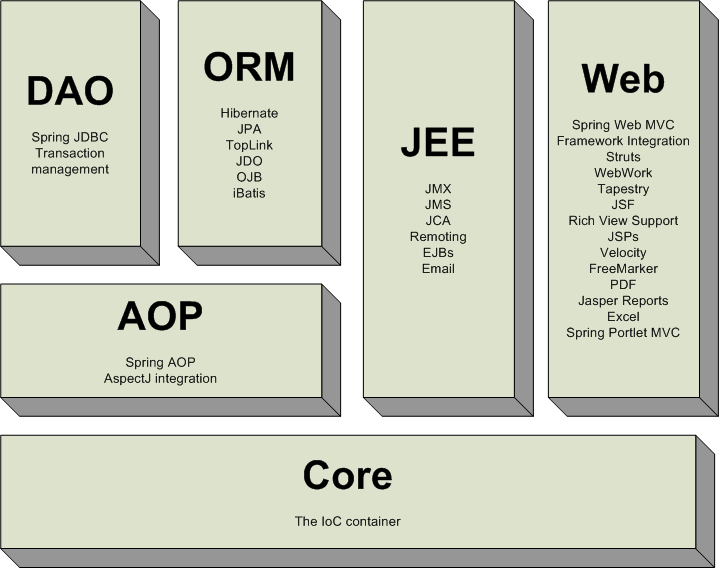
\includegraphics[width=0.9\textwidth]{../spring_framework.png}
    \end{center}
  }

  \frame{\frametitle{Spring Jdbc}
  }

  \frame{\frametitle{MVC}
  }

  \frame{\frametitle{Spring webmvc}
  }

  \frame{\frametitle{ContextLoaderListener}
  }

  \frame{\frametitle{DispatchServlet}
  }

  \frame{\frametitle{元素}
    \begin{itemize}
    \item WebApplicationContext
    \item HandlerMapping
    \item HandlerAdapter
    \item Controller
    \item ModelAndView
    \item ViewResolver
    \item ExceptionResolver
    \end{itemize}
  }

  \frame{\frametitle{启动过程}
      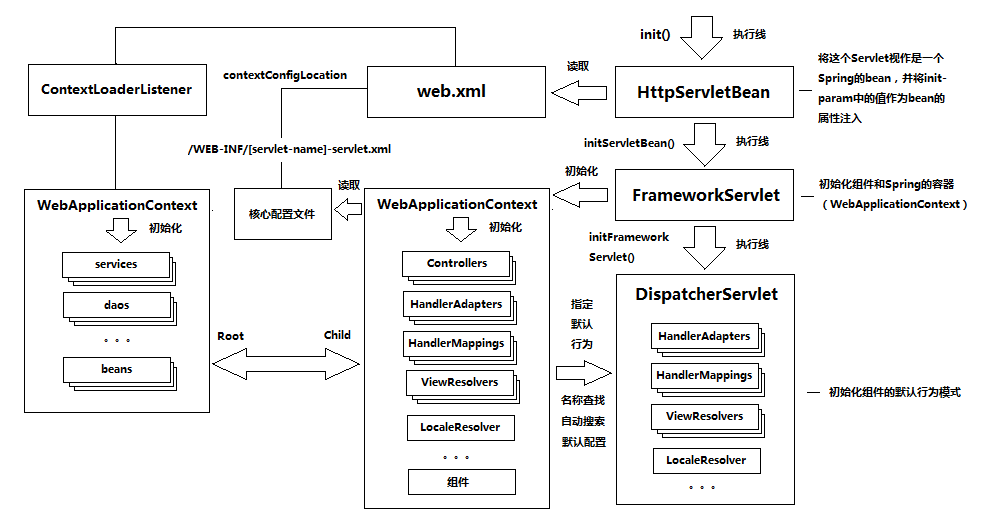
\includegraphics[width=1.1\textwidth]{../spring_init.png}
  }

  % validator
  % locale, message
  % quartz

  \frame{\frametitle{Homework}
  }

  \frame[plain]{
    \begin{center}
      -EOF-
    \end{center}
  }

\end{CJK}
\end{document}
